\begin{enumerate}[label=\thesection.\arabic*.,ref=\thesection.\theenumi]
\numberwithin{equation}{enumi}
\item In a system whose signal flow graph is shown in the figure, $U_1(s)$ and $U_2(s)$ are inputs. The transfer function $\frac{Y(s)}{U_1(s)}$ is

\begin{figure}[!h]
  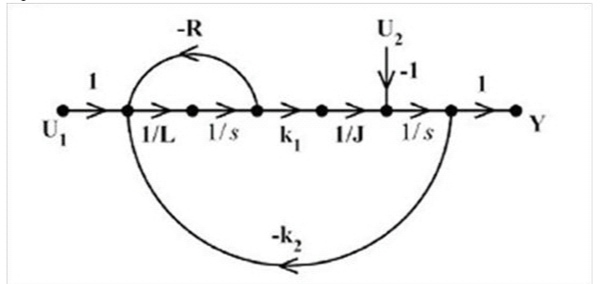
\includegraphics[width=\columnwidth]{image.jpg}
  
\end{figure}



\solution

Masons Gain Formula:

$T=\frac{C(s)}{R(s)}=\frac{\sum_{i=1}^{N}P_i \Delta_i }{\Delta}$

where,
\begin{itemize}
    \item T is the transfer function or the gain between R(s) and C(s)
    \item C(s) is the output node
    \item R(s) is the input node
    \item $P_i$ is the i\textsuperscript{th} forward path gain
    \item $\Delta= 1 - $(sum of all individual loop gains)+(sum of gain products of all possible two non touching loops)-(sum of gain products of all possible three non touching loops)+.... 
    \item $\Delta_i$ is obtained from $\Delta$ by removing the loops which are touching the i\textsuperscript{th} forward path  
     
    
    
\end{itemize}


\begin{align}
\dfrac{Y(s)}{U_1(s)}\Biggr|_{U_2(s)=0}
\end{align}

\begin{align}
P_1=1\cdot\dfrac{1}{L}\cdot\dfrac{1}{s}\cdot k_1 \cdot\dfrac{1}{J}\cdot\dfrac{1}{s}\cdot1=\dfrac{k_1}{LJs^2}
\end{align}

After removing the loops that are touching the forward path, the system will have no loops .Therefore,
\begin{align}
\Delta_1 =1    
\end{align} 



$\Delta= 1 - $(sum of all individual loop gains)
as in this system there are no non touching loops.
Let $L_1$ and $L_2$ be the individual loops.

\centering
$\Delta= 1 - (L_1+L_2)$

\begin{align}
L_1= \dfrac{1}{L}\cdot \dfrac {1}{s}\cdot(-R)=\dfrac{-R}{Ls}
\end{align}


\begin{align}
L_2=\dfrac{1}{L}\cdot \dfrac{1}{s}\cdot k_1 \cdot \dfrac{1}{J} \cdot \dfrac{1}{s}\cdot -(k_2) =\dfrac{-k_2 k_1}{LJs^2}
\end{align}


\begin{align}
\frac{Y(s)}{U_1(s)} = \frac{P_1 \Delta_1}{1-(L_1+L_2)}=\dfrac{\dfrac{k_1}{s^2LJ}}{1+\dfrac{R}{Ls}+\dfrac{k_2 k_1}{LJs^2}}
\end{align}

\centering
\begin{align}
\frac{Y(s)}{U_1(s)}=\frac{k_1}{s^2LJ+sRJ+K_1k_2}
\end{align}


\end{enumerate}